\documentclass{gmcm2026}
\graphicspath{{./}}
\begin{document}
\pagestyle{empty}
\renewcommand{\thefigure}{5.\arabic{figure}}% 本页唯一 figure 图号 5.1，对应交付图 fig-5-1
\setlength{\textfloatsep}{8pt plus 2pt minus 2pt}
\setlength{\abovecaptionskip}{4pt}
% 实际插入宽度 148mm（正文宽 165mm 的 89.7%）：图高 1032/711*148 = 214.8mm
% + 图注 + 浮动间距，实测单页容纳（当前有效口径：148mm，与已交付 PDF 一致）
\begin{figure}[!htbp]
\centering
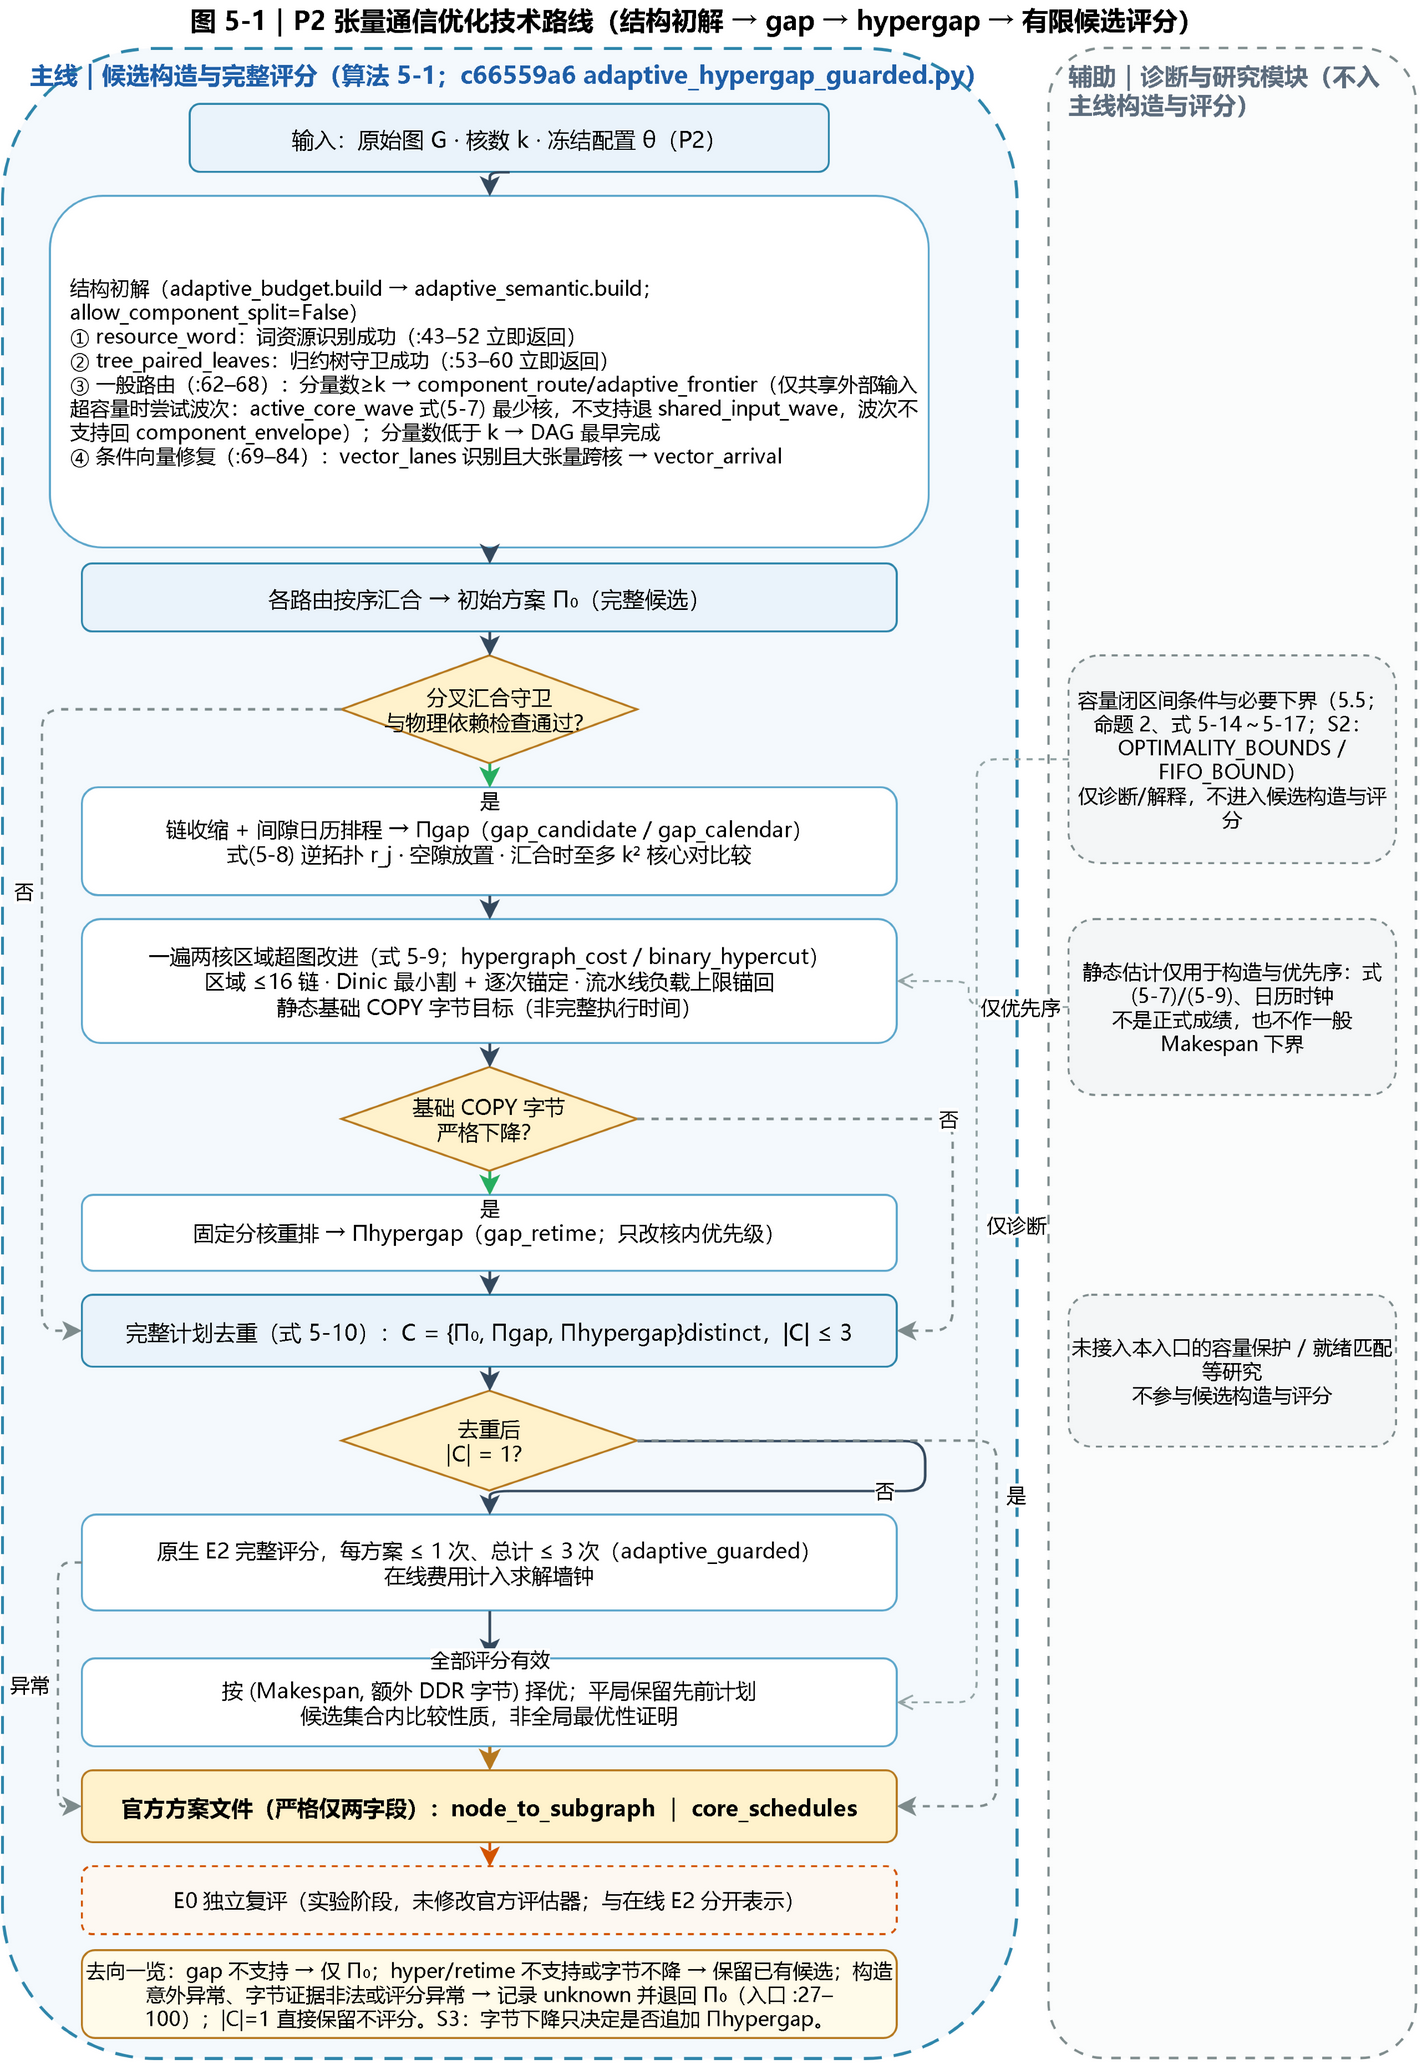
\includegraphics[width=148mm]{fig5-1-p2-tensor-comm-route.png}
\caption{P2 张量通信优化技术路线：结构初解 $\Pi_0$（含式~(5-7) 活跃核选择与条件向量
通路修复）$\to$ 分叉汇合守卫 $\to$ $\Pi_{\mathrm{gap}}$ $\to$ 两核区域超图改进 $\to$ 字节判定 $\to$
$\Pi_{\mathrm{hypergap}}$ $\to$ 去重（$|C|\le3$）$\to$ E2 评分择优（异常退回 $\Pi_0$）$\to$ 两字段方案 $\to$ E0 复评；
侧栏为诊断与研究模块。结构与方法流程图，不声称实测加速或零 spill。}
\end{figure}
\end{document}
